\documentclass[10pt,a4paper]{article}

\usepackage{graphicx}
\usepackage[left=2cm,right=2cm,top=2cm,bottom=2cm]{geometry}
\usepackage[usenames,dvipsnames,svgnames,table]{xcolor}
\usepackage{placeins}

\usepackage{circus}

\newenvironment{ttSection}{\ttfamily}{\par}


\begin{document}
\title{Translation Design}
\date{}
\maketitle
%\section{Annotations}

%\begin{itemize}
%\item \texttt{@NonParadigm(type)} : 'data' or 'active'

%\end{itemize}
When it comes to translation, the key difference between Level~1 and Level~2 programs is the ability to nest mission sequencers inside missions, which creates a tiered program hierarchy with each mission sequencer spawning a new tier. Each tier is formed of several clusters, each cluster pairing a mission with its schedulables. Each mission in a tier is controlled by a mission sequencer in the tier above. The safelet and the top-level mission sequencers are contained in the control tier at the top of the hierarchy. As an example of the tiers within a program, we consider the example in Figure~\ref{fig:AircraftDiagram}, which shows a program controlling an aircraft that has three modes of operation: take off, cruising, and landing.

\begin{figure}[!h]
\begin{center}
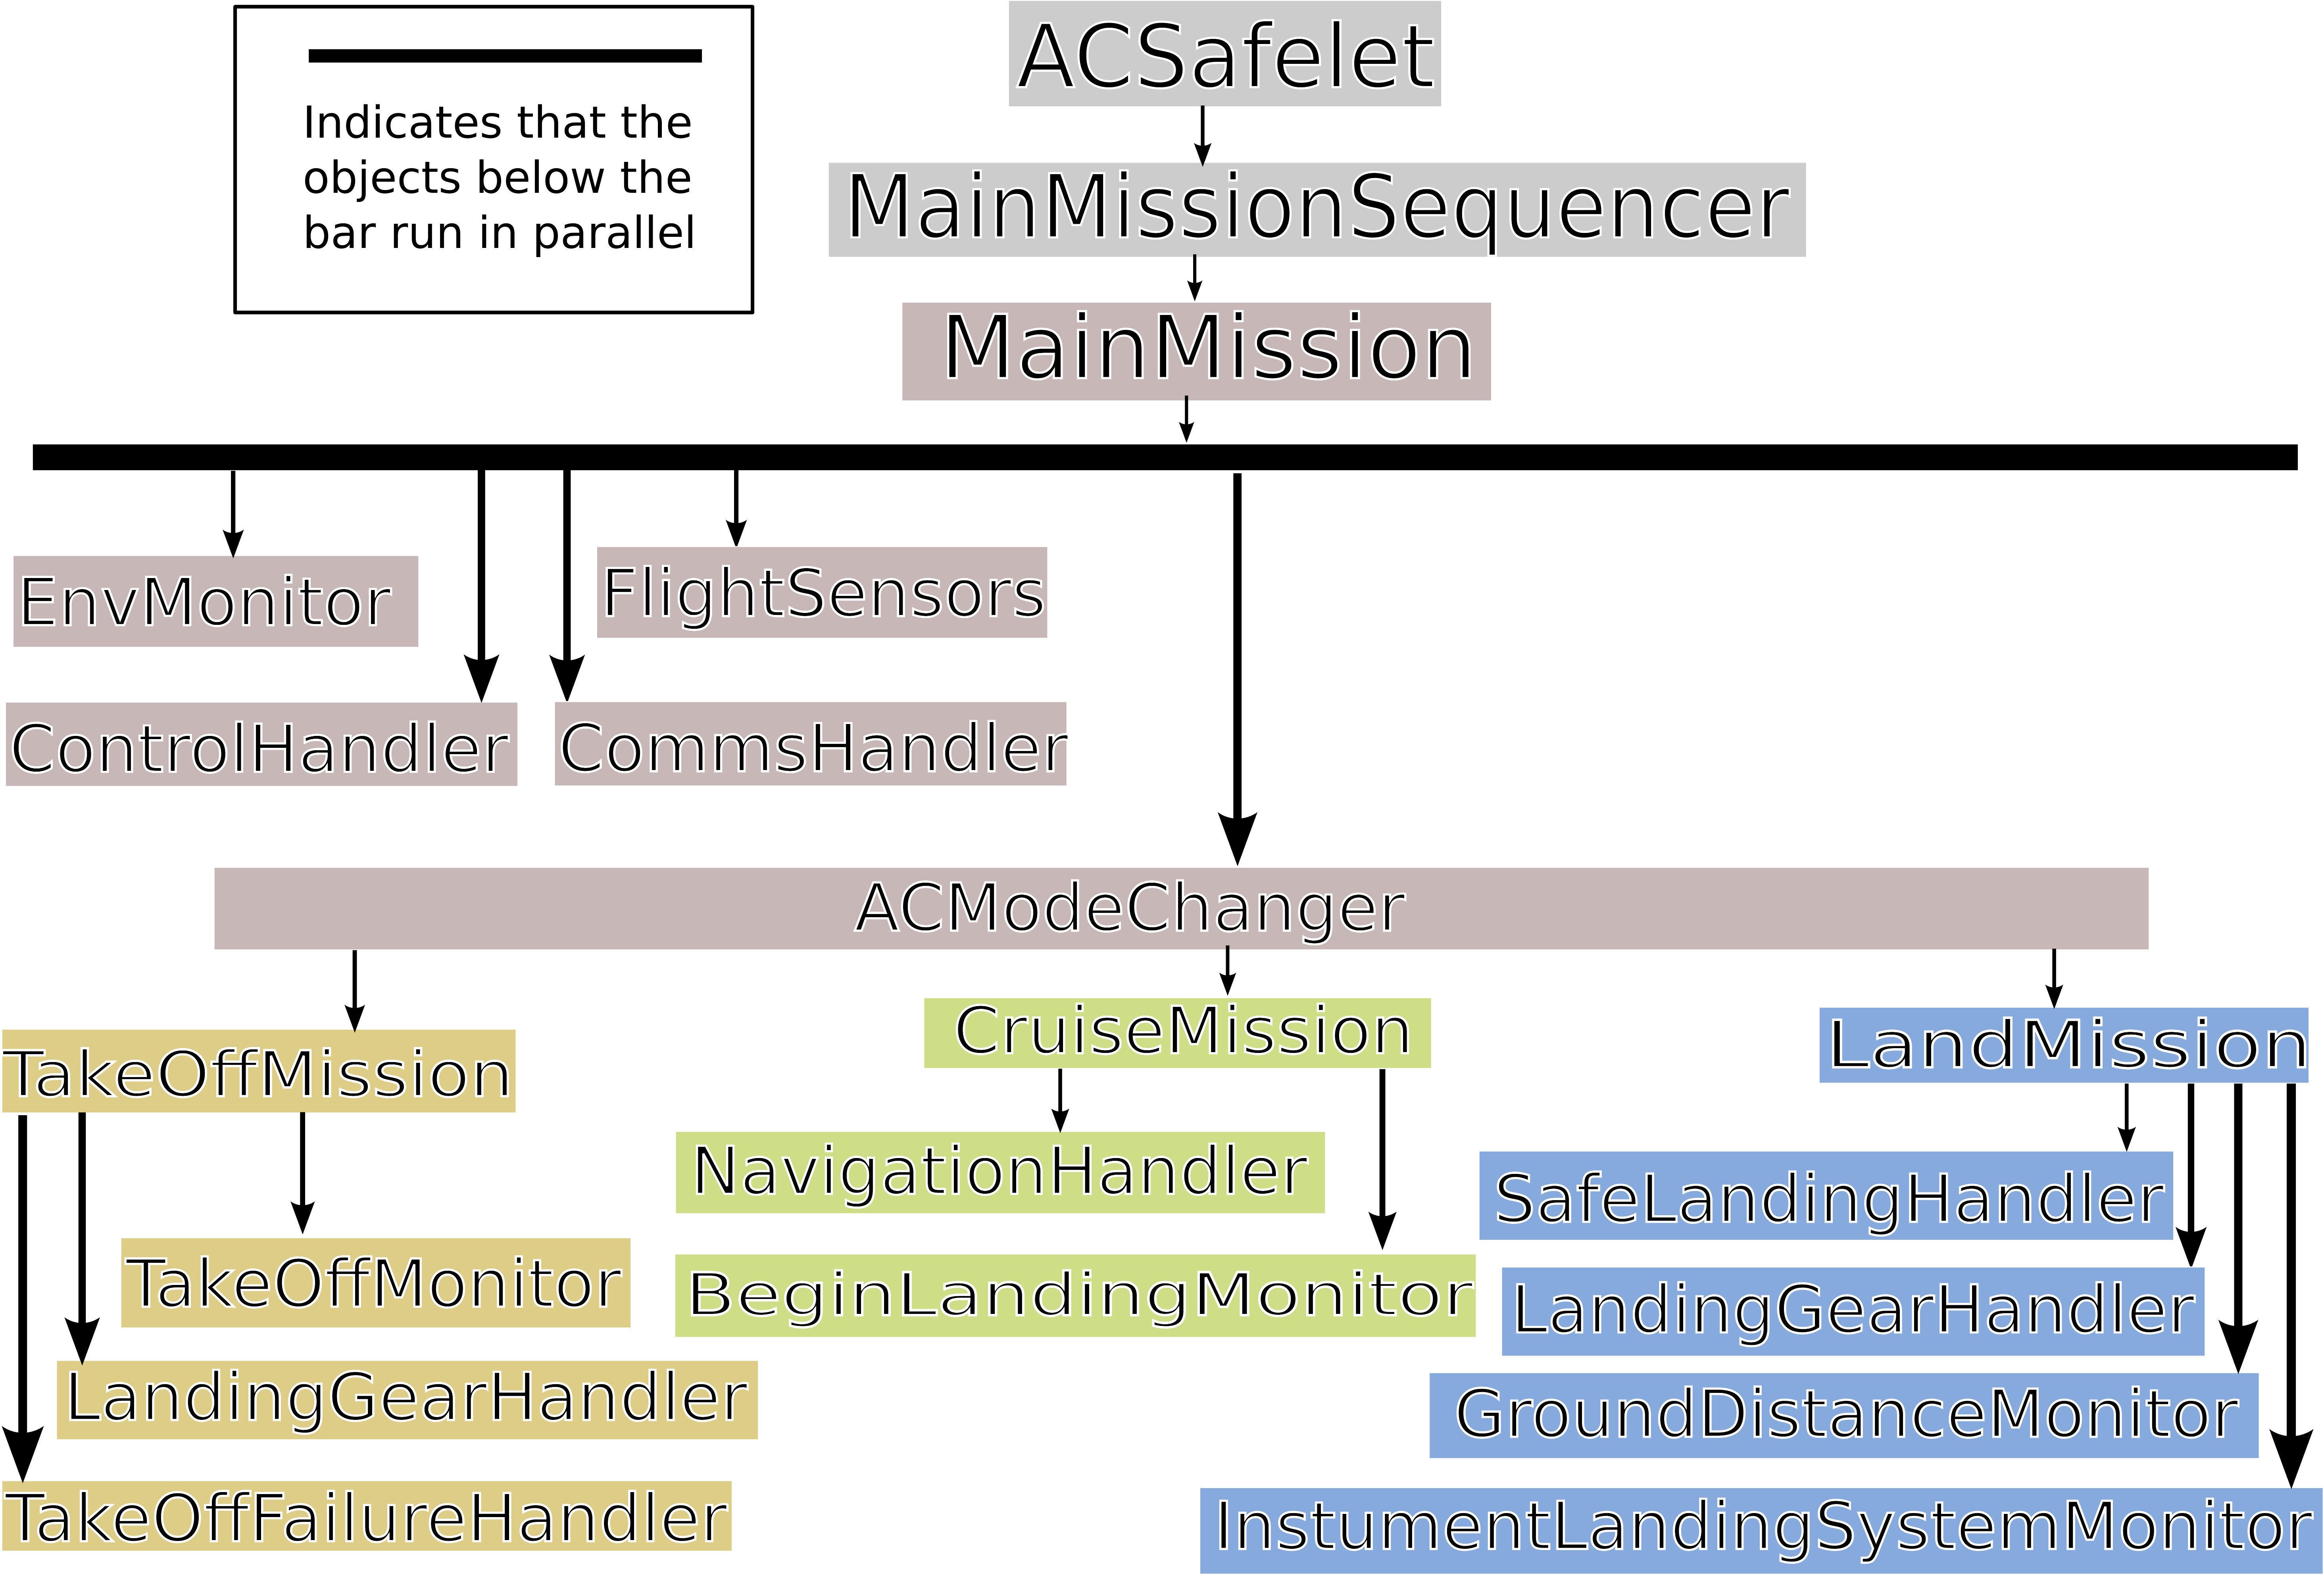
\includegraphics[scale=1]{AircraftStructure.png}
\caption{The hierarchy of classes in a program controlling an aircraft with multiple modes of operation. \label{fig:AircraftDiagram}}
\end{center}
\end{figure}

In this example, the control~tier contains the \texttt{ACSafelet} and \texttt{MainMissionSequencer} classes. Tier~0 contains one cluster that pairs the \texttt{MainMission} with the the four event handlers (\texttt{EnvMonitor}, \texttt{FlightSensors}, \texttt{ControlHandler}, \texttt{CommsHandler}) and the \texttt{ACModeChanger}, which is the nested mission sequencer. This nested mission sequencer indicates that this program has another tier, tier~1.

Tier~1 contains three clusters. Each cluster pairs a single mission with the schedulable objects that it may register. One cluster pairs the \texttt{TakeOffMission} with the \texttt{TakeOffMonitor}, \texttt{LandingGearHandler}, and \texttt{TakeOffFailureHandler}. The second cluster pairs the \texttt{CruiseMission} with the \texttt{NavigationHandler} and \texttt{BeginLandingMonitor}. The final cluster pairs the \texttt{LandMission} with its schedulables: the \texttt{SafeLandingHandler}, \texttt{LandingGearHandler}, \texttt{GroundDistanceMonitor}, and \texttt{InstrumentLandingSystemMonitor}. 

We approach the translation of Level~2 programs with this hierarchical structure in mind. Figure~\ref{fig:translationFlow} shows a flowchart of the translation process.
\begin{figure}[h!]
\begin{center}
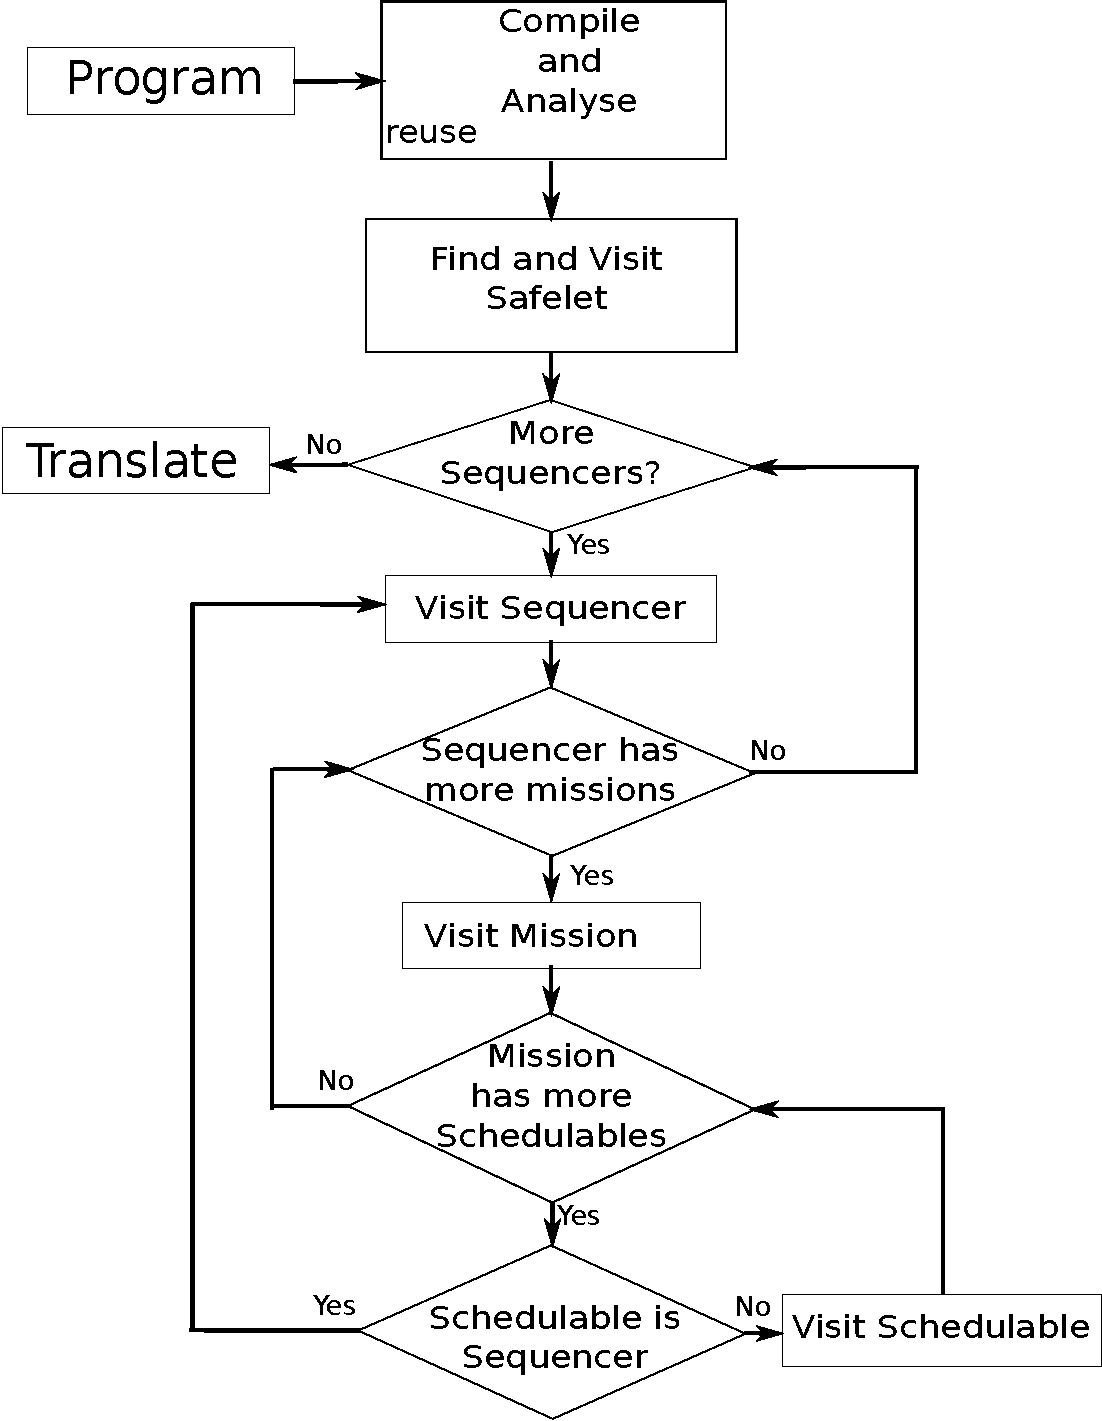
\includegraphics[scale=0.5]{translation.pdf}
\caption{Flowchart of our Translation Process \label{fig:translationFlow} }
\end{center}
\end{figure}
First, We take an SCJ program compile it and analyse it, described briefly in Section~\ref{sec:analysis}. Then we begin the exploration phase, described in Section~\ref{sec:exploration}, in which we extract the information we require from the program. The hierarchy of an SCJ program can be seen as a tree, with the safelet as the root element. The analysis phase, gives us the elements in the program tree, but not its structure, so we start with the safelet and use the objects in the program to build the tree's structure. Once we have explored the tree of objects in the program and extracted the information we need, we proceed to the translation phase -- described in Section~\ref{sec:translation}.

\section{Analysis}
\label{sec:analysis}

In the current tool, the analysis phase takes an SCJ program, compiles it and analyses it using the built-in Java Compiler API. Because the program is compiled using an SCJ implementation, we require that the programs input into our tool are valid SCJ programs that will compile. If compilation errors occur during this phase then the program will not be translated and the tool will show the compilation errors. Further restrictions on the program are required to ensure that the exploration phase can extract the information we require and we describe these in Section~\ref{sec:exploration}.

Since the compilation and analysis of programs is SCJ agnostic, and therefore not tied to any particular compliance level, we intend to reuse this functionality. To check that we can reuse this functionality without causing problems, we have compiled and analysed a simple Level~2 program using the current implementation of the tool. 

The output of this phase is a list of trees the represent the classes in the program. This list of trees is used during the exploration phase, which we describe in the next section.

\section{Exploration}
\label{sec:exploration}

%RESTRICTIONS

Because the analysis phase outputs a representation of each class in the program as tree, we use the visitor pattern to explore the different types of element that we might find in each tree and extract the variables, method contents, and names of the next classes to visit. This phase may make use of some annotations to speed up the discovery of information by packaging it in the annotations instead of requiring the tool to explore the program for it. These annotations are shown in Table~\ref{tab:annotations}.

\begin{tabular}{| l | l | l |}
 Annotation 											& Parameters																										& Used For \\
 \hline
 
 \texttt{@returnsSequencers(names: String[])} 			& \texttt{names} --- an array of the names of the mission sequencers returned by a \texttt{getSequencer()} method 	& A safelet's \texttt{getSequencer()} method \\
 
 \texttt{@returnsMissions(names: String[])} 			& \texttt{names} --- an array of the names of the missions returned by a \texttt{getNextMission()} method			& A mission sequencer's \texttt{getNextMission()} method \\
 
 \texttt{@nonParadigm(type : classType)} 				& \texttt{type} --- the type of non-paradigm object, can be 'data' or 'active'										& Any non-paradigm object \\
 
 \texttt{@createsNonParadigmObject(names : String[])} 	& \texttt{names} --- an array of the names of the non-paradigm objects a method creates								& Any method that creates non-paradigm objects \\
 
 \texttt{@makesNonParadigmMethodCall(names: String[])} 	& \texttt{names} --- an array of the names of the non-paradigm objects a method calls								& Any method that calls a non-paradigm method \\
 
 \texttt{@waits}										& 																													& Any method that calls \texttt{Object.wait()} \\
 
 \texttt{@notifies} 									&																													& Any method that calls \texttt{Object.notify()} \\
 
 \texttt{@callsWaitMethod} 								&																													& Any method that calls a method annotated with \texttt{@waits}\\
 
 \texttt{@callsNotifyMethod} 							&																													& Any method that calls a method annotated with \texttt{@notifies} \\
\end{tabular}


These annotations may be omitted because the method detailed below can extract this information from the program itself. However, including with the annotations makes the exploration phase quicker. We intend to implement exploring annotated programs first, then implement the more complicated methods detailed below.  

The exploration phase is focussed on the paradigm objects, those objects that extend classes or implement interfaces in the SCJ API. Upon discovery, each object (apart from the safelet) is assigned a unique identifier based upon the class's name -- multiple instances of a class result in multiple identifiers. This identifier is used in our model as a parameter to the processes representing that class. The location of the discovered objects within the program is important for the translation and is also recorded.

The safelet can be identified easily because there is only one in the program. We retrieve the possible top-level mission sequencers and then begin a loop in the flow of exploring the program. For each top-level mission sequencer, we explore all of the missions that it can return. In doing so we visit each of a mission's managed schedulables until there are none left and then we return to the previous stage and explore the next mission. If there are no more missions, then we return to the stage above and explore the next mission sequencer. Because we build the tree of an SCJ program depth-first, if there are no more top-level mission sequencers to visit then we have explored the whole program and we can proceed to the translation phase, described in Section~\ref{sec:translation}.

Sections~\ref{sec:safelet} to~\ref{sec:schedulables} detail the methodology for each stage of the exploration phase, while Section~\ref{sec:other} details how we capture other possible program elements. 

\subsection{Find and Visit Safelet}
\label{sec:safelet}

Because there is only one safelet in a program, to find the program's safelet we search the list of class trees returned by the analysis phase and identify the class that implements \texttt{javax.safetycritical.Safelet}. Once the safelet is identified, we visit it and extract the contents of the \texttt{initializeApplication()} and \texttt{getSequencer()} methods, as well as any program-defined methods and variables. 

The \texttt{getSequencer()} method returns classes that extend \texttt{javax.safetycritical.MissionSequencer}. These classes are the top-level mission sequencers and their names are collected and visited in the next stage of the translation. 

Finally, the name of the safelet class is recorded for use in the translation of the high-level network of the processes in the model. Next we visit the top-level mission sequencers.

\subsection{Visit Sequencer}
\label{sec:sequencer}
This stage makes use of the top-level sequencer names recorded as the return values from the safelet's \texttt{getSequencer()} method, it is also used to translate any nested mission sequencers that are found during the visiting of schedulables. We discus nested mission sequencers further in Section~\ref{sec:schedulables}.

When visiting either flavour of mission sequencer we capture the contents of the \texttt{getNextMission()} method and any program-specific methods and variables. We collect the return values of the \texttt{getNextMission()} method, which returns classes that extend \texttt{javax.safetycritical.Mission}, for use in the next stage of the translation. 

Finally, we record the name of this sequencer and its location in the hierarchy. If it is returned by the safelet's \texttt{getSequencer()} method, then is is a top-level sequencer. If it is returned by a mission, then it is a nested mission sequencer. 

\subsection{Visit Mission}
\label{sec:mission}

This translation stage makes use of the collected names of the missions returned by the \texttt{getNextMission()} method of a mission sequencer. We visit each mission returned by a particular mission sequencer and each of that mission's schedulables before moving on to the next mission. This is because we pair each mission with its schedulables to form a cluster. 

When visiting a mission we capture the contents of the \texttt{initialize()} and \texttt{cleanUp()} methods, as well as any program-specific methods and variables. To find the schedulables of a mission we find any class that may be registered during the mission's \texttt{initialize()} method. The names of these classes are collected and used in the next stage of the translation. 

We record the name of this mission, in preparation for pairing it with its schedulables as a cluster. We also record where in the hierarchy this mission resides. For example, if it is returned by a top-level mission sequencer, then it resides in tier 0. 

\subsection{Visit Schedulable}
\label{sec:schedulables}

This stage of the translation takes a collection of names of the schedulables registered in a mission's \texttt{initialize()} method. We visit each schedulable in turn; if the schedulable extends \texttt{javax.safetycritical.MissionSequencer}, then we use the same method described in Section~\ref{sec:sequencer}. Otherwise, we check if the schedulable is a managed thread or one of the three kinds of event handler, again by checking what class the schedulable extends, and proceed.

When visiting a nested mission sequencer we visit the mission sequencer and then begin visiting its missions and their schedulables. A nested mission sequencer indicates a new tier in the program's hierarchy. When visiting a schedulable that isn't a mission sequencer, we capture the \texttt{handleAsyncEvent()} method of event handlers or the \texttt{run()} method of managed threads, as well as any program-specific methods and variables. Finally, we record each schedulable’s position and pair it with its mission.

\subsection{Other Considerations}
\label{sec:other}

\subsubsection{Non-Paradigm Objects}

Non-paradigm objects are objects in the program that do not extend classes or implement interfaces from the SCJ API. During the hierarchical exploration of the program, if we find the instantiation of any non-paradigm objects then they are visited to collect any variables and the contents of their methods. The names of these objects are recorded separately and are translated using a template specific to non-paradigm objects.

\subsubsection{Components making Non-paradigm Method Calls}

A non-paradigm method call is a call to a method that is declared in the program, not in the infrastructure of SCJ. Because we need to model them differently, we must identify when components make non-paradigm method calls. They can only occur during program-specific code, so we check each method called in application code to see if the class in which the method is declared is in the SCJ API or not. 

For example, to check for non-paradigm method calls in the application code of a mission, we check each method call in its \texttt{initialize()} and \texttt{cleanUp()} methods. If the method called is declared in a class that is not \texttt{javax.safetycritical.Mission} then it is record it as non-paradigm method call. 


\subsubsection{Wait and Notify}

Once of the features unique to SCJ Level~2 is the ability to use Java suspension with the \texttt{Object.wait()} and \texttt{Object.notify()} methods. To wait on an object a thread must hold the lock of that object. In SCJ this can only occur by calling a \texttt{synchronized} method. Further, SCJ restricts calls to the suspension methods so that they can only be called on \texttt{this}. This means that for a schedulable object to wait on some shared data object, it must call a synchronised method that wraps the call to \texttt{Object.wait()}. Similarly, calls to \texttt{Object.notify()} on that shared data object must be wrapped in a \texttt{synchronized} method. 

While exploring the program, if we find a synchronised method which calls \texttt{Object.wait()} or \texttt{Object.notify()} we record its name. If we later find an object that calls this method, we can establish the relationship between these two object, that one is waiting on the other, or that one is calling notify on the other. Suspension is likely to occur between schedulable objects and objects in the mission memory area above those schedulable objects. However, as this is not a restriction of the SCJ paradigm we may need to make another pass of the program to fully detect and use of suspension.


\section{Translate}
\label{sec:translation}

The translation phase occurs in two stages. The low-level translation takes the information gathered about each of the classes in the program during the exploration phase and produces the application and framework processes that represent them in our model, for example the safeletApp and safeletFW processes. The high-level translation translates the information gathered about the program hierarchy and translates it into the clusters and tiers that make up the network of processes at the top-level of our model. This network takes the form $Application \interleave Framework$, where $Framework$ contains the framework processes arranged as a hierarchy according to the information found during the exploration phase and $Application$ contains the application processes and any program-specific method calls. 

Both stages of the translation are achieved using the Freemarker template engine, which takes a data model and a template and combines them to produce output. For the low-level translation, the information gathered from visiting each class in the program (as we described in Section~\ref{sec:exploration}) is used to produce a data model for that class. The relevant template is loaded and combined with the data model to produce our model. For the high-level translation, the information record by each visitor about the position in the hierarchy of the class it is visiting is used to construct a data model of the tiers and clusters that make up the program, this is combined with the template for the network to produce the high-level network that controls the processes in our model.


\end{document}